\documentclass[11pt]{article}

\usepackage[margin=1in]{geometry}
\usepackage{tikz}
\usetikzlibrary{arrows.meta, positioning, shapes.geometric, fit}
\usepackage{booktabs}
\usepackage{array}
\usepackage{listings}
\usepackage{xcolor}
\usepackage{hyperref}
\usepackage{enumitem}
\usepackage{caption}
\usepackage{parskip}

\lstset{
  basicstyle=\ttfamily\small,
  breaklines=true,
  columns=fullflexible,
  frame=single,
  backgroundcolor=\color{gray!7},
  showstringspaces=false
}

\hypersetup{colorlinks=true, linkcolor=blue, urlcolor=blue, citecolor=blue}

\title{\vspace{-1.5cm}Design Report \\ Tool 9: Dictionary Attack and Known Password Attack}
\author{}
\date{}

\begin{document}
\maketitle
\vspace{-2.5cm}

\begin{center}
\begin{tabular}{ll}
\textbf{Course:} & CSE406 \\
\textbf{Deadline:} & 11th Week \\
\end{tabular}
\end{center}

\begin{table}[h!]
\centering
\begin{tabular}{lll}
\toprule
\textbf{Member} & \textbf{Student ID} & \textbf{Responsibility} \\
\midrule
\rule{0pt}{2.2ex}\underline{\hspace{4cm}} & \underline{\hspace{2.5cm}} & Webapp (\texttt{app.py}, \texttt{db.py}) + defense (\texttt{defense.py}) \\[1.2ex]
\underline{\hspace{4cm}} & \underline{\hspace{2.5cm}} & Attacker tools + report diagrams \\
\bottomrule
\end{tabular}
\caption*{Fill in names/IDs before submitting.}
\end{table}

\section*{a. Definition of the Attack, with Topology Diagram}

\subsection*{Dictionary attack}
The attacker targets \emph{one specific account} and tries a large ordered list of
candidate passwords (a ``dictionary'' of common/likely passwords) against it, one at a
time, until the server accepts one or the list is exhausted. The attack works because
many users choose passwords that appear in common wordlists.

\subsection*{Known password attack (password spraying / credential reuse)}
The attacker instead starts from a small set of \emph{known} passwords --- defaults,
previously breached passwords, or passwords obtained from another attack (e.g.\
sniffing) --- and tries each one against a \emph{wide list of accounts}. This exploits
password reuse and default credentials rather than weak individual passwords, and is
harder to detect with a naive per-account lockout, since no single account receives
many failed attempts.

Both attacks target a small signup/login web application built from scratch
(\texttt{src/app.py}, Flask + SQLite). The victim is a basic webapp with a real
signup/login/database, not an existing service such as SSH or FTP. The \emph{victim
action} is a normal user signing up and logging in through a browser; the
\emph{attacker action} is the two attacks above, driven by our own HTTP client code
(\texttt{attacker\_dict.py}, \texttt{attacker\_spray.py}) --- not an existing
brute-forcing tool such as Hydra or Medusa.

\subsection*{Topology}

\begin{figure}[h!]
\centering
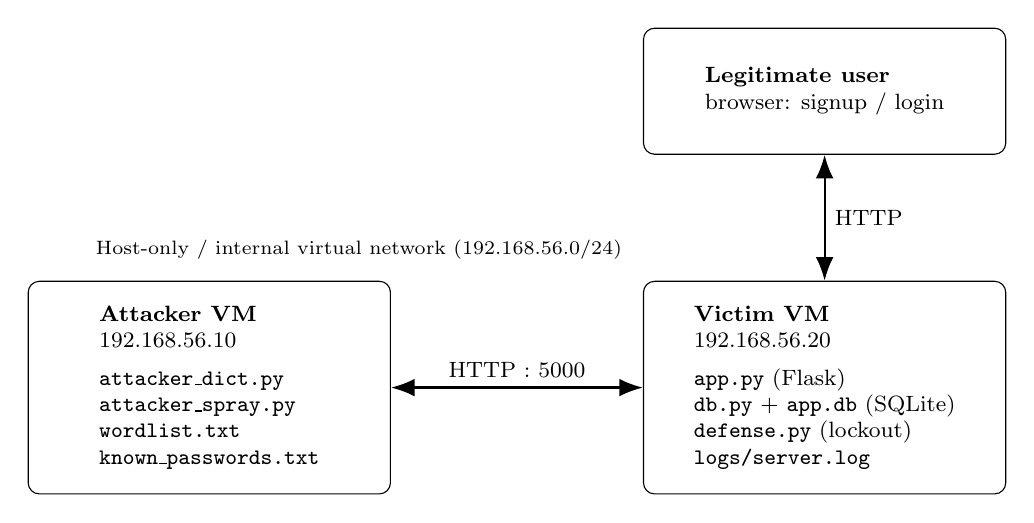
\begin{tikzpicture}[
  box/.style={draw, rectangle, rounded corners, align=left, minimum width=4.6cm,
              minimum height=2.7cm, font=\footnotesize, inner sep=8pt},
  node distance=2.2cm
]
\node[box] (attacker)
  {\textbf{Attacker VM} \\ 192.168.56.10 \\[4pt]
   \texttt{attacker\_dict.py} \\ \texttt{attacker\_spray.py} \\
   \texttt{wordlist.txt} \\ \texttt{known\_passwords.txt}};

\node[box, right=3.2cm of attacker] (victim)
  {\textbf{Victim VM} \\ 192.168.56.20 \\[4pt]
   \texttt{app.py} (Flask) \\ \texttt{db.py} + \texttt{app.db} (SQLite) \\
   \texttt{defense.py} (lockout) \\ \texttt{logs/server.log}};

\node[box, above=1.6cm of victim, minimum height=1.6cm] (user)
  {\textbf{Legitimate user} \\ browser: signup / login};

\draw[{Latex[length=3mm]}-{Latex[length=3mm]}, thick]
  (attacker) -- node[above, font=\footnotesize]{HTTP : 5000} (victim);
\draw[{Latex[length=3mm]}-{Latex[length=3mm]}, thick]
  (user) -- node[right, font=\footnotesize]{HTTP} (victim);

\node[font=\scriptsize, align=center, above=0.15cm of attacker, xshift=1.9cm]
  {Host-only / internal virtual network (192.168.56.0/24)};
\end{tikzpicture}
\caption{Attack topology: two VMs on a host-only virtual network, plus a legitimate
browser client exercising the same webapp.}
\end{figure}

\emph{Replace the placeholder IPs with your actual VirtualBox host-only subnet once the
VMs are set up, and attach an \texttt{ip addr} screenshot from both VMs.}

\section*{b. Timing Diagrams}

\subsection*{Normal (legitimate) signup + login --- browser flow}

\begin{figure}[h!]
\centering
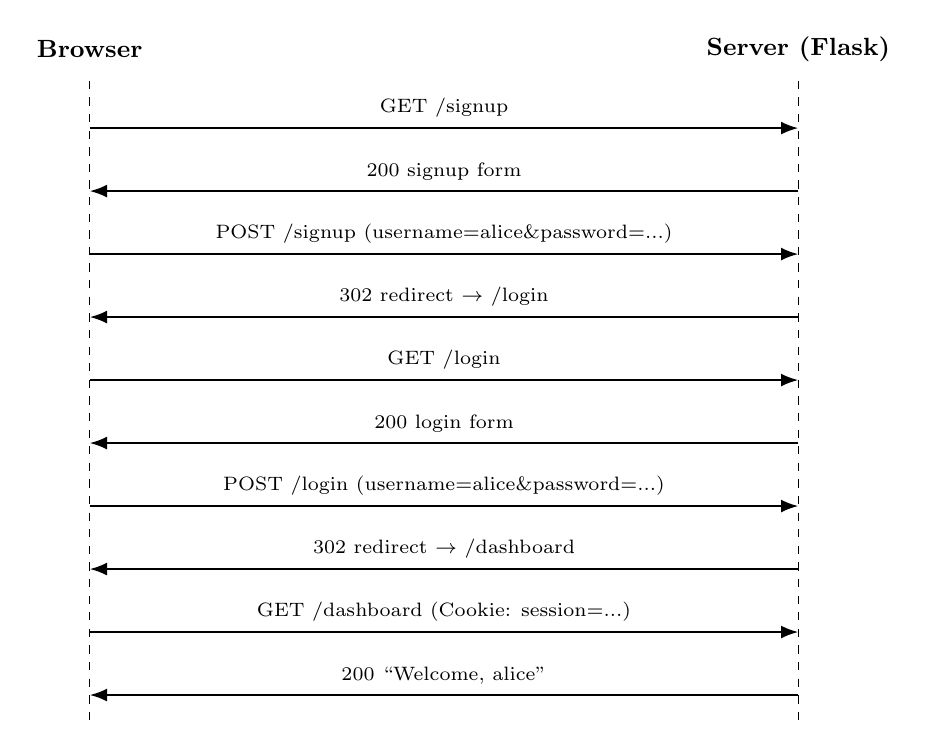
\begin{tikzpicture}[
  msg/.style={-{Latex[length=2.2mm]}, thick},
  lbl/.style={font=\scriptsize, midway, above}
]
\node[font=\bfseries\small] at (0,0.4) {Browser};
\node[font=\bfseries\small] at (9,0.4) {Server (Flask)};
\draw[dashed] (0,0) -- (0,-8.2);
\draw[dashed] (9,0) -- (9,-8.2);

\draw[msg] (0,-0.6)  -- (9,-0.6)  node[lbl]{GET /signup};
\draw[msg] (9,-1.4)  -- (0,-1.4)  node[lbl]{200 signup form};
\draw[msg] (0,-2.2)  -- (9,-2.2)  node[lbl]{POST /signup (username=alice\&password=...)};
\draw[msg] (9,-3.0)  -- (0,-3.0)  node[lbl]{302 redirect $\rightarrow$ /login};
\draw[msg] (0,-3.8)  -- (9,-3.8)  node[lbl]{GET /login};
\draw[msg] (9,-4.6)  -- (0,-4.6)  node[lbl]{200 login form};
\draw[msg] (0,-5.4)  -- (9,-5.4)  node[lbl]{POST /login (username=alice\&password=...)};
\draw[msg] (9,-6.2)  -- (0,-6.2)  node[lbl]{302 redirect $\rightarrow$ /dashboard};
\draw[msg] (0,-7.0)  -- (9,-7.0)  node[lbl]{GET /dashboard (Cookie: session=...)};
\draw[msg] (9,-7.8)  -- (0,-7.8)  node[lbl]{200 ``Welcome, alice''};
\end{tikzpicture}
\caption{Normal protocol timing: one legitimate signup followed by one login.}
\end{figure}

\subsection*{Dictionary attack --- repeated exchange, one account}

\begin{figure}[h!]
\centering
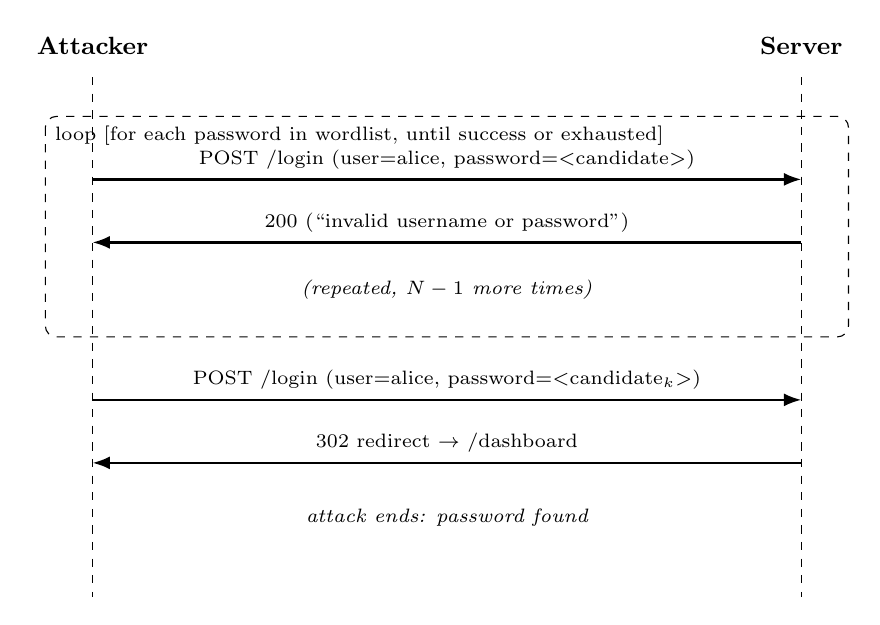
\begin{tikzpicture}[
  msg/.style={-{Latex[length=2.2mm]}, thick},
  lbl/.style={font=\scriptsize, midway, above}
]
\node[font=\bfseries\small] at (0,0.4) {Attacker};
\node[font=\bfseries\small] at (9,0.4) {Server};
\draw[dashed] (0,0) -- (0,-6.6);
\draw[dashed] (9,0) -- (9,-6.6);

\draw[dashed, rounded corners] (-0.6,-0.5) rectangle (9.6,-3.3);
\node[font=\scriptsize, anchor=north west] at (-0.6,-0.5)
  {loop~[for each password in wordlist, until success or exhausted]};

\draw[msg] (0,-1.3) -- (9,-1.3) node[lbl]{POST /login (user=alice, password=\textless candidate\textgreater)};
\draw[msg] (9,-2.1) -- (0,-2.1) node[lbl]{200 (``invalid username or password'')};
\node[font=\scriptsize\itshape] at (4.5,-2.7) {(repeated, $N-1$ more times)};

\draw[msg] (0,-4.1) -- (9,-4.1) node[lbl]{POST /login (user=alice, password=\textless candidate$_k$\textgreater)};
\draw[msg] (9,-4.9) -- (0,-4.9) node[lbl]{302 redirect $\rightarrow$ /dashboard};
\node[font=\scriptsize\itshape] at (4.5,-5.6) {attack ends: password found};
\end{tikzpicture}
\caption{Dictionary attack: many candidate passwords tried in sequence against a single account.}
\end{figure}

\subsection*{Known-password (spray) attack --- repeated exchange, many accounts}

\begin{figure}[h!]
\centering
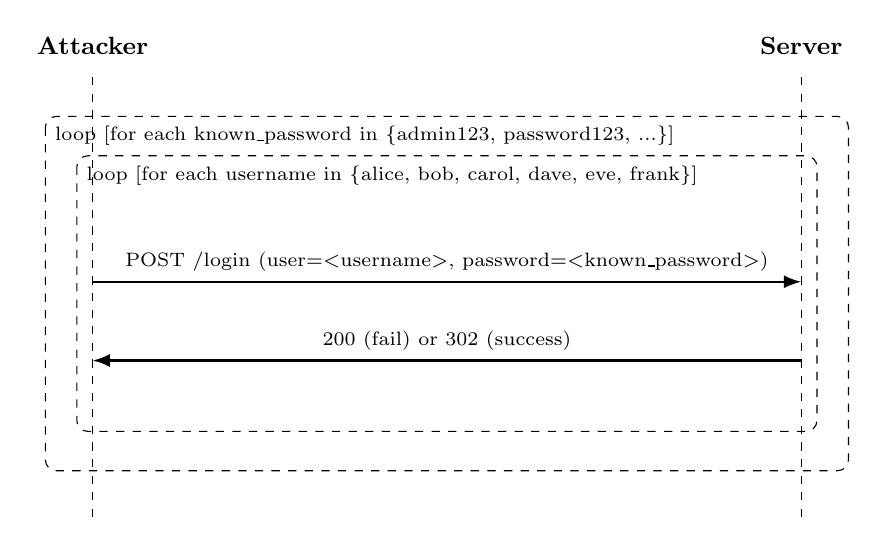
\begin{tikzpicture}[
  msg/.style={-{Latex[length=2.2mm]}, thick},
  lbl/.style={font=\scriptsize, midway, above}
]
\node[font=\bfseries\small] at (0,0.4) {Attacker};
\node[font=\bfseries\small] at (9,0.4) {Server};
\draw[dashed] (0,0) -- (0,-5.6);
\draw[dashed] (9,0) -- (9,-5.6);

\draw[dashed, rounded corners] (-0.6,-0.5) rectangle (9.6,-5.0);
\node[font=\scriptsize, anchor=north west] at (-0.6,-0.5)
  {loop~[for each known\_password in \{admin123, password123, ...\}]};

\draw[dashed, rounded corners] (-0.2,-1.0) rectangle (9.2,-4.5);
\node[font=\scriptsize, anchor=north west] at (-0.2,-1.0)
  {loop~[for each username in \{alice, bob, carol, dave, eve, frank\}]};

\draw[msg] (0,-2.6) -- (9,-2.6) node[lbl]{POST /login (user=\textless username\textgreater, password=\textless known\_password\textgreater)};
\draw[msg] (9,-3.6) -- (0,-3.6) node[lbl]{200 (fail) or 302 (success)};
\end{tikzpicture}
\caption{Known-password / spray attack: few known passwords tried across many accounts.}
\end{figure}

\subsection*{With the lockout defense active}

\begin{figure}[h!]
\centering
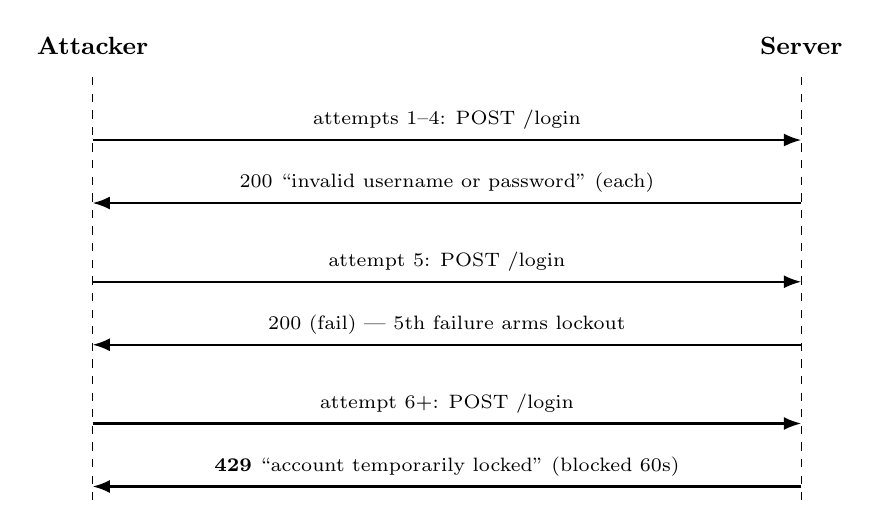
\begin{tikzpicture}[
  msg/.style={-{Latex[length=2.2mm]}, thick},
  lbl/.style={font=\scriptsize, midway, above}
]
\node[font=\bfseries\small] at (0,0.4) {Attacker};
\node[font=\bfseries\small] at (9,0.4) {Server};
\draw[dashed] (0,0) -- (0,-5.4);
\draw[dashed] (9,0) -- (9,-5.4);

\draw[msg] (0,-0.8) -- (9,-0.8) node[lbl]{attempts 1--4: POST /login};
\draw[msg] (9,-1.6) -- (0,-1.6) node[lbl]{200 ``invalid username or password'' (each)};

\draw[msg] (0,-2.6) -- (9,-2.6) node[lbl]{attempt 5: POST /login};
\draw[msg] (9,-3.4) -- (0,-3.4) node[lbl]{200 (fail) --- 5th failure arms lockout};

\draw[msg] (0,-4.4) -- (9,-4.4) node[lbl]{attempt 6+: POST /login};
\draw[msg] (9,-5.2) -- (0,-5.2) node[lbl]{\textbf{429} ``account temporarily locked'' (blocked 60s)};
\end{tikzpicture}
\caption{Lockout defense: the dictionary/spray attack is blocked after 5 failed attempts
within a 30-second window.}
\end{figure}

\section*{c. Packet / Frame / Segment Details}

Transport is standard TCP carrying HTTP/1.1 (Flask's built-in development server); no
raw Ethernet/IP crafting is needed for this attack class, since the exploit is at the
application layer. What was designed from scratch is the \emph{application behaviour
and payload} the HTTP request carries, and how the server interprets it --- not an
existing authentication protocol implementation.

\subsection*{Request (attacker or browser $\rightarrow$ server), one per login attempt}

\begin{lstlisting}
POST /login HTTP/1.1
Host: 192.168.56.20:5000
Content-Type: application/x-www-form-urlencoded
Content-Length: 33

username=alice&password=sunshine
\end{lstlisting}

\subsection*{Responses, by outcome}

\begin{table}[h!]
\centering
\begin{tabular}{lll}
\toprule
\textbf{Outcome} & \textbf{Status} & \textbf{Notable headers / body} \\
\midrule
Success & \texttt{302 FOUND} & \texttt{Location: /dashboard}, \texttt{Set-Cookie: session=...} \\
Failure & \texttt{200 OK} & login page HTML containing ``invalid username or password'' \\
Locked (defense on) & \texttt{429 TOO MANY REQUESTS} & login page HTML containing ``account temporarily locked'' \\
\bottomrule
\end{tabular}
\end{table}

\subsection*{Design notes to include with packet captures}

\begin{itemize}[leftmargin=*]
  \item Each attempt opens its own TCP connection (the attacker scripts issue a plain
    \texttt{requests.post()} call per attempt, with no session reuse) --- a full 3-way
    handshake, HTTP request/response, then FIN/ACK teardown per attempt. Capture this
    in Wireshark and annotate source/destination port, sequence numbers, and the HTTP
    payload of each segment (\emph{Follow $>$ HTTP Stream} is the easiest way to show
    this in the report).
  \item The response to a failed login is intentionally the same generic ``invalid
    username or password'' whether the username does not exist or the password is
    wrong --- the app does not leak account existence. Constant-shape hashing
    (\texttt{db.py}, \texttt{verify\_user}) additionally hashes against a dummy salt
    when the username does not exist, so a nonexistent-user request does not return
    measurably faster than a wrong-password request.
  \item Server-side credential storage: \texttt{salt (16 bytes) + SHA-256(salt +
    password)} in undefended mode; \texttt{salt + PBKDF2-HMAC-SHA256(password, salt,
    200000 iterations)} in defended mode.
  \item Passwords are sent as cleartext form data over plain HTTP in this demo (no
    TLS) --- a deliberate simplification consistent with the assignment's other
    plaintext-protocol attacks (e.g.\ Tool 2's Telnet/HTTP sniffing), and worth noting
    as a limitation versus a production deployment, which would use HTTPS.
\end{itemize}

\section*{d. Justification}

\begin{itemize}[leftmargin=*]
  \item The victim accounts are deliberately seeded with passwords drawn from
    \texttt{wordlist.txt} (\texttt{alice}, \texttt{bob}, \texttt{carol}), so the
    dictionary attack is expected to succeed within the first few dozen attempts ---
    measured locally: \texttt{alice} cracked in 17/50 attempts ($\approx$0.03\,s,
    undefended).
  \item \texttt{eve} and \texttt{frank} share a common default password
    (\texttt{admin123}) that also exists in \texttt{known\_passwords.txt}, so the
    spray attack is expected to compromise both without needing a large wordlist
    against either account individually --- validated in local testing (2/6 accounts
    compromised in one spray pass).
  \item \texttt{dave} uses a high-entropy password absent from both lists and is
    expected to resist both attacks --- this is the negative control, demonstrating
    that the attacks fail against passwords that are not guessable from common lists,
    rather than the tool being broken.
  \item Without rate limiting, an attacker can attempt logins as fast as the
    network/CPU allows, making a wordlist of any realistic size crackable in seconds.
    This justifies why the lockout + slow-hash countermeasure is necessary and
    measurably effective.
\end{itemize}

\begin{table}[h!]
\centering
\begin{tabular}{lcc}
\toprule
& \textbf{Undefended} & \textbf{Defended (\texttt{DEFENSE=1})} \\
\midrule
Cost per login attempt & $\approx$1--2\,ms (SHA-256) & $\approx$55\,ms (PBKDF2, 200k iter.) \\
Dictionary attack on \texttt{alice} & cracked, 17 attempts, 0.03\,s & locked out, 6 attempts, 0.27\,s \\
Spray attack outcome & 2/6 accounts compromised & attempts throttled per account \\
\bottomrule
\end{tabular}
\caption{Measured before/after effect of the lockout + slow-hash countermeasure (local
single-host test; re-measure on the two-VM setup before submitting).}
\end{table}

\bigskip
\noindent\textbf{TODO before submission:} insert VM IP addresses and an \texttt{ip
addr} screenshot from both VMs; insert a Wireshark capture screenshot with 2--3
annotated HTTP request/response pairs (and a ``Follow HTTP Stream'' view); insert a
browser screenshot of a normal signup + login + dashboard flow as the victim-action
evidence; re-measure the numbers in Section~d on the actual two-VM setup and update the
table above.

\end{document}
